%%
%%  ISG@UP Lab Book Document Class.
%%  Copyright (C) 2014-2022, University of Pretoria.
%%

%% Control directives for rubber LaTeX build system
% rubber: makeidx.style isglabbook.ist

\documentclass[11pt,a4paper]{isglabbook}

%% Document specific overrides.
\newcommand{\doctype}{Lab Book}
\newcommand{\docauthor}{Mitchell Luke Williams}
\newcommand{\docstudentnumber}{18013555}

%% Configure PDF information
\hypersetup{
  pdftitle={\doctype},
  pdfauthor={\docauthor\ - \docstudentnumber},
  pdfsubject={\eeceup},
  pdfkeywords={\doctype}
}

%% Switch to package specific header/footer format
\pagestyle{fancyisg}

% Code listing setup

\usepackage{listings}
\usepackage{color}

\definecolor{dkgreen}{rgb}{0,0.6,0}
\definecolor{gray}{rgb}{0.5,0.5,0.5}
\definecolor{mauve}{rgb}{0.58,0,0.82}

\lstset{frame=tb,
   language=Python,
   aboveskip=3mm,
   belowskip=3mm,
   showstringspaces=false,
   columns=flexible,
   basicstyle={\small\ttfamily},
   numbers=none,
   numberstyle=\tiny\color{gray},
   keywordstyle=\color{blue},
   commentstyle=\color{dkgreen},
   stringstyle=\color{mauve},
   breaklines=true,
   breakatwhitespace=true
   tabsize=3
   }

\begin{document}
\pagenumbering{arabic}

% Front Matter
%%
%%  ISG@UP General Document Front Page Template
%%  Copyright (C) 2014-2022, University of Pretoria.
%%

\thispagestyle{empty}
{
  \renewcommand{\baselinestretch}{1.2}
  \newcommand{\HRule}{\rule{\linewidth}{0.4mm}}
  \setlength{\parindent}{0mm}
  \setlength{\parskip}{0mm}
  \pagfamily{}
  \centering

  \begin{figure*}[!ht]
    \centering
\includegraphics[width=10cm]{up-logo.eps}
  \end{figure*}

  \medskip
  {\sc\Large\bchfamily Faculty of Engineering, Built Environment \\
    and Information Technology} \\
  \medskip
  \medskip
  {\sc\large\sffamily \eece}
  \url{http://www.up.ac.za/eece}

  \vspace*{\stretch{1}}

  {\Large\bfseries\MakeUppercase{\doctype}}

  \vspace*{\stretch{1}}

  {\slshape Compiled by} \\
  \medskip
  \medskip
  {\large\bfseries\docauthor} \\
  {\large\docstudentnumber}

  \vspace*{\stretch{0.5}}
  {\slshape Generated on}\\
  \medskip
  \medskip
  {\bfseries \today}

  \vspace*{\stretch{1}}

  {\Huge\lmssfamily\bfseries ISG@UP} \\
  {\bfseries \sc \Large Intelligent Systems Group} \\
  \url{http://isg.up.ac.za/} \\
}

%% End of File.


% Table / Lists
\pdfbookmark[1]{Contents}{sec:toc}
{\small\cmbrfamily\tableofcontents}
\newpage

%% Document Body
\renewcommand{\baselinestretch}{1.5}
\subimport{2022/}{202203}
\subimport{2022/}{202204}
\subimport{2022/}{202205}
\subimport{2022/}{202206}
\subimport{2022/}{202207}
\subimport{2022/}{202208}
\subimport{2022/}{202209}
\subimport{2022/}{202210}
% \subimport{2022/}{202211}

%% Appendices
\newpage
\appendix
\appendixpage
\addappheadtotoc
%%
%%  ISG@UP Lab Book - General Acronyms
%%  Copyright (C) 2014-2022, University of Pretoria.
%%

\section{Acronyms}

\begin{acronym}[CSMACD]
  \acro{AI}{Artificial Intelligence}
  \acro{ANN}{Artificial Neural Network}
  \acro{BIC}{Bayesian Information Criterion}
  \acro{CRF}{Conditional Random Field}
  \acro{CRFs}{Conditional Random Fields}
  \acro{CVPR}{Computer Vision and Pattern Recognition}
  \acro{dB}{decibel}
  \acro{DBN}{dynamic Bayesian network}
  \acro{EBIT}{Faculty of Engineering, Built Environment and Information Technology}
  \acro{ECCV}{European Conference on Computer Vision}
  \acro{EECE}{Department of Electrical, Electronic and Computer Engineering}
  \acro{EKF}{Extended Kalman Filter}
  \acro{EM}{Expectation Maximisation}
  \acro{FFNN}{feed-forward neural network}
  \acro{FFT}{Fast Fourier Transform}
  \acro{FOV}{Field Of View}
  \acro{fps}{Frames per second}
  \acro{FPU}{Floating Point Unit}
  \acro{FSM}{Finite State Machine}
  \acro{GA}{Genetic Algorithm}
  \acro{GAs}{Genetic Algorithms}
  \acro{GD}{Gradient Descent}
  \acro{GMs}{graphical models}
  \acro{GNU}{Recursive Acronym: GNU's Not Unix}
  \acro{GP}{Gaussian Process}
  \acro{GPs}{Gaussian Processes}
  \acro{GPL}{General Public Licence}
  \acro{GUI}{Graphical Users Interface}
  \acro{HMM}{Hidden Markov Model}
  \acro{HMMs}{Hidden Markov Models}
  \acro{HVS}{human visual system}
  \acro{ICA}{Independent Component Analysis}
  \acro{ICCV}{International Conference on Computer Vision}
  \acro{ICRA}{International Conference on Robotics and Automation}
  \acro{IEEE}{Institute of Electrical and Electronics Engineers}
  \acro{IROS}{Intelligent Robots and Systems}
  \acro{LUT}{lookup table}
  \acro{MC}{Monte Carlo methods}
  \acro{MDP}{Markov Decision Process}
  \acro{MDS}{multi-dimensional scaling}
  \acro{MIT}{Massachusetts Institute of Technology}
  \acro{ML}{machine learning}
  \acro{MLE}{maximum likelihood estimation}
  \acro{PCA}{Principle Component Analysis}
  \acro{POMDP}{Partially Observable Markov Decision Process}
  \acro{PSO}{Particle Swarm Optimisation}
  \acro{PV}{Pixel Value}
  \acro{RANSAC}{Random Sample Consensus}
  \acro{RGB}{Red Green Blue}
  \acro{RNG}{random number generator}
  \acro{RNGs}{random number generators}
  \acro{ROI}{Region of Interest}
  \acro{RPROP}{Resilient Propagation}
  \acro{RSS}{residual sums of squares}
  \acro{SA}{Simulated Annealing}
  \acro{SLAM}{Simultaneous localization and mapping}
  \acro{SSE}{Sum Squared Error}
  \acro{SVD}{Singular Value Decomposition}
  \acro{SVM}{Support Vector Machine}
  \acro{SVMs}{Support Vector Machines}
  \acro{UP}{University of Pretoria}
\end{acronym}

\pendsign
\newpage

%% End of File.


\begin{figure}[h]
  \centering
  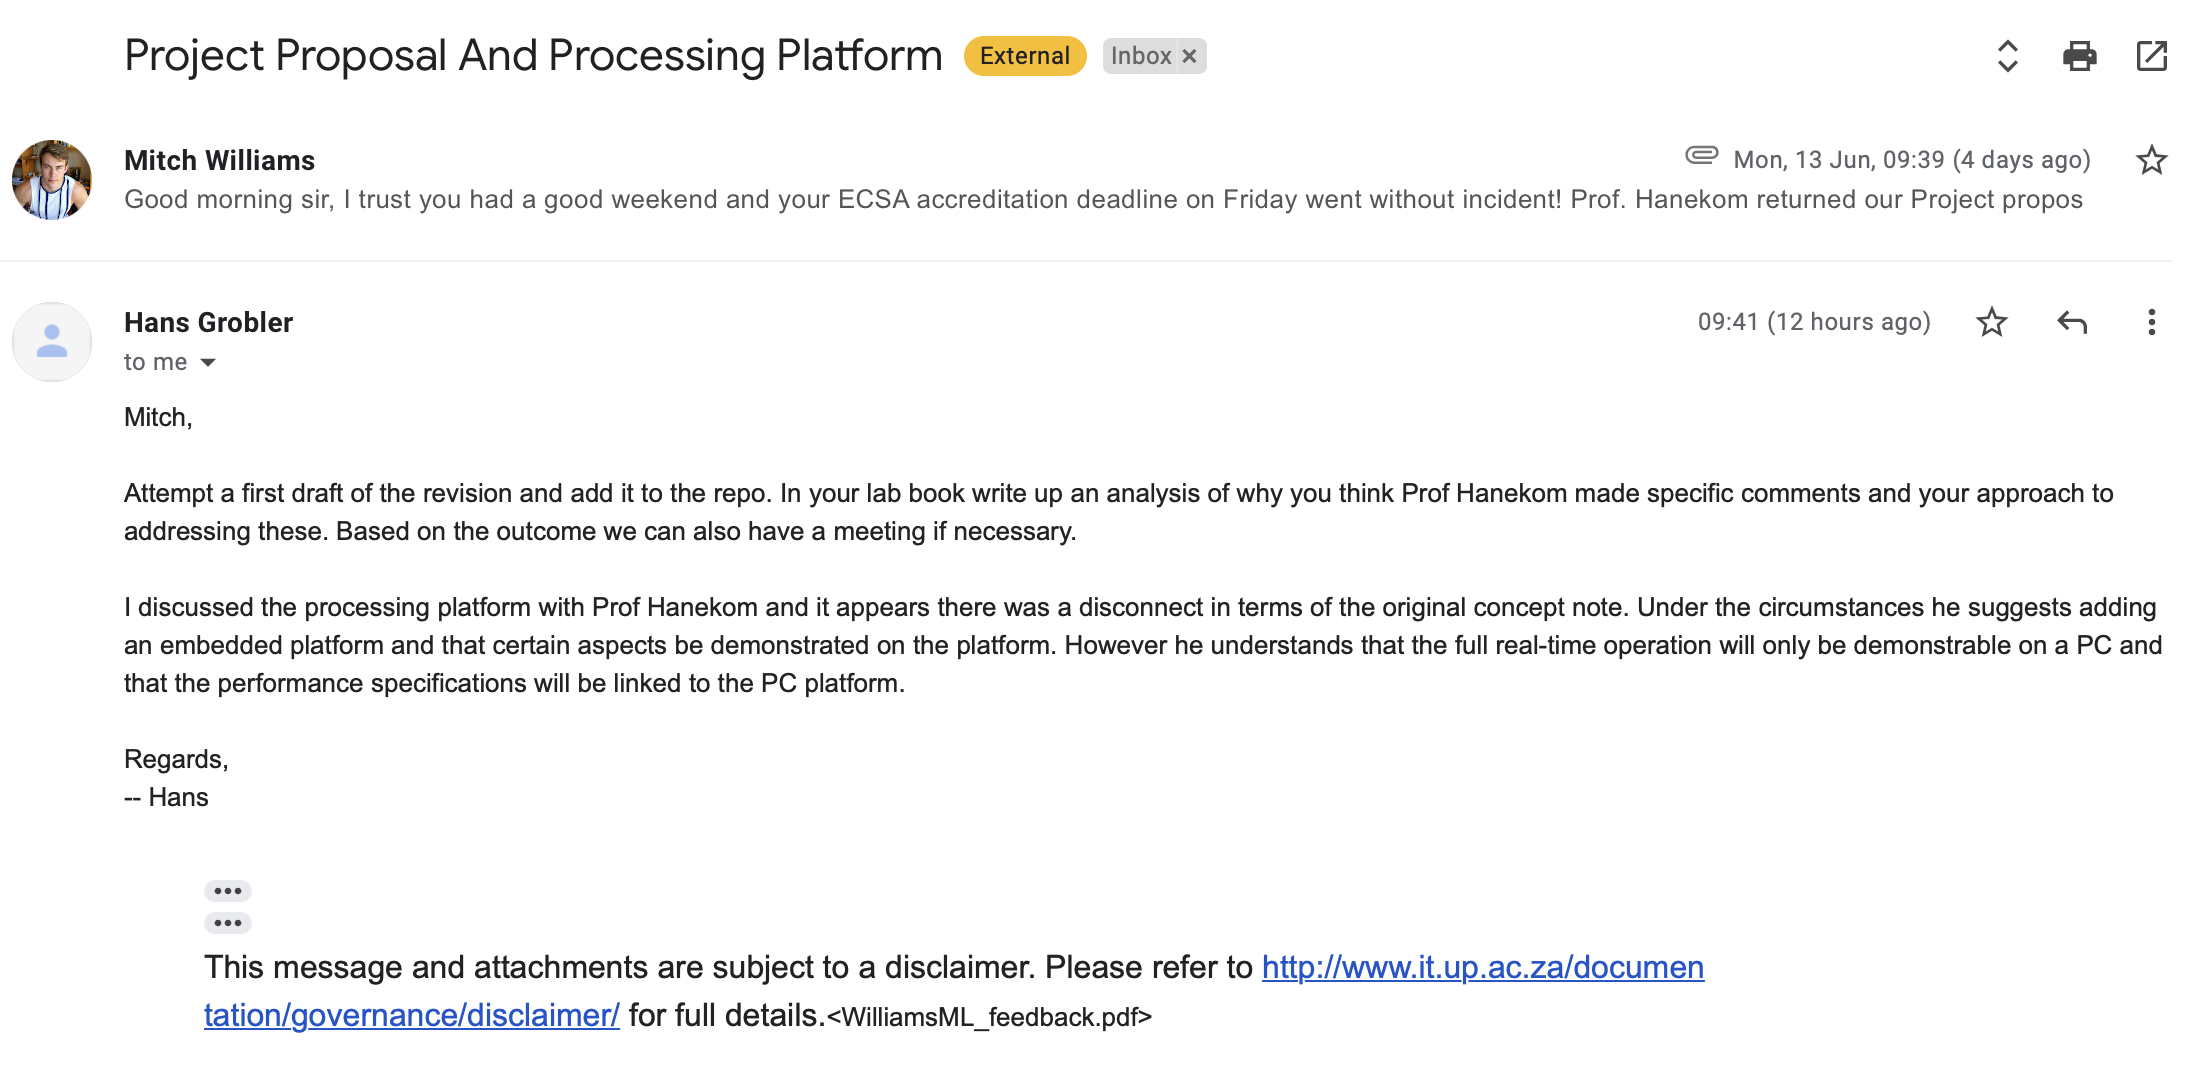
\includegraphics[width=0.9\linewidth]{2022/figures/appendix/email_embedded.png}
  \caption{Email dated Friday 17 June 2022 between Mr. Grobler and Mr. Williams}
  \label{fig:grobler_email}
\end{figure}


%% Bibliography
\newpage
\addcontentsline{toc}{chapter}{References}
\bibliographystyle{ieeetr}
\bibliography{references}

%% Back Matter / Index
\newpage
\addcontentsline{toc}{chapter}{Index}
\printindex

%% The End
\end{document}

%% End of File.
